\documentclass[abstract=on,10pt,a4paper,bibliography=totocnumbered]{article}
\usepackage[paper=a4paper,left=35mm,right=35mm,top=25mm,bottom=30mm]{geometry}
\usepackage[doublespacing]{setspace}
\usepackage[english]{babel}
\usepackage[utf8]{inputenc}
\usepackage{amsmath}
\usepackage{colortbl}
\usepackage{amsfonts}
\usepackage{amssymb}
\usepackage{gensymb}
\usepackage{textcomp}
\usepackage{graphicx}
\usepackage{tikz}
\usepackage{enumerate}
\usepackage{enumitem}
\usepackage{subcaption}
\usepackage{booktabs}
\usepackage[hidelinks]{hyperref}
\usepackage[nameinlink]{cleveref}
\usepackage{multirow}
\usepackage{arydshln}
\usepackage[flushleft]{threeparttable}
\usepackage[nomarkers, nolists]{endfloat}
\usepackage{scalerel}
\usepackage{makecell}
\usepackage{ifthen}
\usepackage{tikz}
\usepackage{lineno}
\usetikzlibrary{svg.path}

%------------------------------------------------------------------------------
%  Bibtex vs Biblatex
%------------------------------------------------------------------------------
% While bibtex is very nice to use, it's insanely slow. I therefore work with
% bibtex until the final stage. Set the value below to "true" or "false" to pick
% which one should be used.
\newboolean{usebiblatex}
\setboolean{usebiblatex}{false}

% Depending on the question, the commands below will prepare the document
% accordingly
\ifthenelse{\boolean{usebiblatex}}{
  %-----------------------------------------------------------------------------
  %  If using biblatex
  %-----------------------------------------------------------------------------
  % Load required packages and refer to correct bibliography
  \usepackage{csquotes}
  \usepackage[
      backend=biber
    , style=apa          % To display Author-year in the text
    , natbib=true        % Necessary to use citep, etc.
    , hyperref=true      % To have clickable links in the references
    , useeditor=false    % Don't add editor to publications
    , sorting=ynt        % Sort by year, name, and title
    , uniquename=false   % Avoid that initials are put
  ]{biblatex}
  \addbibresource{Literature.bib}

  % To include author in link
  \DeclareFieldFormat{citehyperref}{%
  \DeclareFieldAlias{bibhyperref}{noformat}% Avoid nested links
  \bibhyperref{#1}}
  \DeclareFieldFormat{textcitehyperref}{%
  \DeclareFieldAlias{bibhyperref}{noformat}% Avoid nested links
  \bibhyperref{%
    #1%
    \ifbool{cbx:parens}
      {\bibcloseparen\global\boolfalse{cbx:parens}}
      {}}}
  \savebibmacro{cite}
  \savebibmacro{textcite}
  \renewbibmacro*{cite}{%
    \printtext[citehyperref]{%
      \restorebibmacro{cite}%
      \usebibmacro{cite}}}
  \renewbibmacro*{textcite}{%
    \ifboolexpr{
      ( not test {\iffieldundef{prenote}} and
        test {\ifnumequal{\value{citecount}}{1}} )
      or
      ( not test {\iffieldundef{postnote}} and
        test {\ifnumequal{\value{citecount}}{\value{citetotal}}} )
    }
      {\DeclareFieldAlias{textcitehyperref}{noformat}}
      {}%
    \printtext[textcitehyperref]{%
      \restorebibmacro{textcite}%
      \usebibmacro{textcite}}}

  % Remove editor form everything but books
  \AtEveryBibitem{%
   \ifentrytype{book}{}{%
    \clearname{editor}
   }
  }
}{
  %-----------------------------------------------------------------------------
  %  If using bibtex
  %-----------------------------------------------------------------------------
  % Load required packages and select citation style
  \usepackage[round]{natbib}
  \bibliographystyle{apalike}
}

%------------------------------------------------------------------------------
%	Some Styling
%------------------------------------------------------------------------------
% Link colors
\definecolor{linkcolor}{HTML}{000000}
\hypersetup{
  colorlinks = true,
  linkcolor  = linkcolor,
  urlcolor   = linkcolor,
  citecolor  = linkcolor,
}

% Changing the style of captions in figures etc.
\captionsetup{labelfont=bf, format=plain, font=small}

% Change how equations are referenced
\renewcommand{\theequation}{Equation \arabic{equation}}%

% Avoid skip when including text from external .tex file
\newcommand{\inputy}[1]{\input{#1}\unskip}

% For supplementary material
\newcommand{\beginappendix}{%
  \setcounter{table}{0}
  \renewcommand{\thetable}{S\arabic{table}}%
  \setcounter{figure}{0}
  \renewcommand{\thefigure}{S\arabic{figure}}%
  \setcounter{equation}{0}
  \renewcommand{\theequation}{Equation S\arabic{equation}}%
  \setcounter{section}{0}
  \renewcommand{\thesection}{A.\arabic{section}}%
}

%------------------------------------------------------------------------------
%  ORCID
%------------------------------------------------------------------------------
% Creating some TikZ styles
\tikzset{
  nonterminal/.style = {rectangle
    , minimum size = 6mm
    , very thick
    , draw = black!
  }
}

% Create the ORCID logo
\definecolor{orcidlogocol}{HTML}{A6CE39}
\tikzset{
  orcidlogo/.pic={
    \fill[orcidlogocol]
      svg{M256,128c0,70.7-57.3,128-128,128C57.3,256,0,198.7,0,128C0,57.3,57.3
        ,0,128,0C198.7,0,256,57.3,256,128z};
    \fill[white]
      svg{M86.3,186.2H70.9V79.1h15.4v48.4V186.2z}
      svg{M108.9,79.1h41.6c39.6,0,57,28.3,57,53.6c0,27.5-21.5,53.6-56.8
        ,53.6h-41.8V79.1z M124.3,172.4h24.5c34.9,0,42.9-26.5
        ,42.9-39.7c0-21.5-13.7-39.7-43.7-39.7h-23.7V172.4z}
      svg{M88.7,56.8c0,5.5-4.5,10.1-10.1,10.1c-5.6,0-10.1-4.6-10.1-10.1c0-5.6
      ,4.5-10.1,10.1-10.1C84.2,46.7,88.7,51.3,88.7,56.8z};
  }
}

% Command to create the ORCID
\newcommand\orcid[1]{\href{https://orcid.org/#1}{\mbox{\scalerel*{

\begin{tikzpicture}[yscale=-1,transform shape]
  \pic{orcidlogo};
\end{tikzpicture}
}{|}}}}

%------------------------------------------------------------------------------
%	Titlepage: Header
%------------------------------------------------------------------------------
\title{Simulating Dispersal across Seasonal Landscapes to Assess Dynamic
Connectivity for an Endangered Large Carnivore}

% List of Authors
\author{
  David D. Hofmann\textsuperscript{1,2,\S} \orcid{0000-0003-3477-4365} \and
  Dominik M. Behr\textsuperscript{1,2} \orcid{0000-0001-7378-8538} \and
  John W. McNutt\textsuperscript{2} \and
  Arpat Ozgul\textsuperscript{1, 2} \orcid{0000-0001-7477-2642} \and
  Gabriele Cozzi\textsuperscript{1,2} \orcid{0000-0002-1744-1940}
}

% Reduce spacing between authors
\makeatletter
\def\and{%
  \end{tabular}%
  \hskip -0.5em \@plus.17fil\relax
  \begin{tabular}[t]{c}}
\makeatother

% Current Date
% \date{\today}

% And here the masterpiece begins
\begin{document}

% Change page numbering
\pagenumbering{gobble}

% Create Titlepage
\maketitle

%------------------------------------------------------------------------------
%	Titlepage: Additional Info
%------------------------------------------------------------------------------
\begin{flushleft}

\vspace{0.5cm}

\textsuperscript{1} Department of Evolutionary Biology and Environmental
Studies, University of Zurich, Winterthurerstrasse 190, 8057 Zurich,
Switzerland.

\textsuperscript{2} Botswana Predator Conservation Program, Wild Entrust,
Private Bag 13, Maun, Botswana.

\textsuperscript{\S} Corresponding author: \href{mailto://david.hofmann2@uzh.ch}{david.hofmann2@uzh.ch}

\vspace{4cm}

\textbf{Running Title:} Seasonality and Landscape Connectivity: Understanding
Nature's Changing Pathways

\vspace{0.5cm}

\textbf{Keywords:} Seasonality, dispersal, connectivity, individual-based,
Lycaon pictus, Okavango Delta

\end{flushleft}

%------------------------------------------------------------------------------
%	Abstract
%------------------------------------------------------------------------------
\newpage
\begin{abstract}

Many ecosystems experience changes in environmental conditions due to
seasonality. While seasonal changes may drastically alter connectivity for
endangered species, most studies represent their system by a static set of
spatial layers, thus ignoring potential changes in environmental conditions due
to seasonal variation. Here, we study seasonal environmental fluctuations
across the Okavango Delta in Botswana and investigate how they affect dispersal
and connectivity for the endangered African wild dog (\textit{Lycaon pictus}).
For this, we compile an extensive set of raster layers accurately representing
seasonal changes in environmental conditions and we combine them with GPS data
collected on dispersing wild dogs to parametrize a dispersal model. Using the
parameterized model, we simulate dispersal trajectories, as environmental
conditions change and we investigate emerging patterns of connectivity. Despite
a better understanding of the conservation needs for African wild dogs, our
study also provides evidence that incorporating seasonality in studies of
connectivity is imperative to more accurately predict the dispersal ability of
endangered species.

\end{abstract}

%------------------------------------------------------------------------------
%	Main Text
%------------------------------------------------------------------------------
\newpage

\onehalfspacing
\tableofcontents
\doublespacing

% Change page numbering
\newpage
\pagenumbering{arabic}

% Create linenumbers
% \linenumbers
\section{Introduction}

Landscape connectivity, i.e. the degree to which a landscape facilitates or
impedes movement among habitat patches \citep{Taylor.1993}, plays a central role
in maintaining biodiversity \citep{Fahrig.2003} and is one of the most
frequently recommended strategies to promote resilience against changing
environmental conditions \citep{Heller.2009, Rudnick.2012}. Studies of landscape
connectivity typically combine information on environmental conditions with
knowledge about species' preferences to delineate critical movement corridors
\citep{Beier.2008, Diniz.2019}. However, while seasonality is a fundamental
characteristic of many ecosystems, it only rarely enters connectivity models in
an explicit manner. Ignoring seasonality, either in environmental conditions or
species' habitat preferences, may result in biased connectivity estimates and a
misallocation of scarce conservation funds \citep{Osipova.2019, Zeller.2020}.

In light of the continued degradation, fragmentation, and destruction of
valuable habitats worldwide \citep{Fahrig.2003, Haddad.2015}, preserving and
reestablishing connectivity between remaining habitat patches has become a task
of utmost importance \citep{Heller.2009, Rudnick.2012}. Improved connectivity
facilitates dispersal \citep{Doerr.2011, Baguette.2013}, i.e. the movement of
individuals away from their natal location to the site of first reproduction
\citep{Clobert.2012}, which in turn promotes genetic diversity
\citep{Perrin.2000, Frankham.2002} and the colonization of vacant habitats
\citep{Hanski.1999, MacArthur.2001}. Two popular approaches to estimate
connectivity are least-cost path analysis \citep{Adriaensen.2003} and circuit
theory \citep{McRae.2008}, both graph-based methods that quantify conductance of
the landscape based on a resistance surface \citep{Zeller.2012, Diniz.2019}.
More recently, individual-based movement models (IBMMs), where dispersal is
explicitly simulated based on a set of movement rules, have been proposed as a
powerful and flexible alternative to graph-based analyses \citep{Kanagaraj.2013,
Allen.2016, Hauenstein.2019, Diniz.2019, Zeller.2020, UnnithanKumar.2022a,
UnnithanKumar.2022, Hofmann.2023}.

Recent advancements in remote sensing technologies and an increasingly
facilitated access to petabytes of landscape data at unprecedented spatial and
temporal scales have created new opportunities to study seasonality and its
impacts on connectivity \citep{Toth.2016, Rumiano.2020}. Google Earth Engine,
for instance, is an online catalog and cloud-based analysis platform that
facilitates a standardized and fully reproducible workflow to explore,
manipulate, analyze, and download a broad range of satellite products that
readily capture seasonal changes across the globe \citep{Zhao.2021}.
Furthermore, the ability to complete computationally demanding processing steps
on Google servers permits such data to be processed using average computers.
Simultaneously, the downsizing of GPS tracking devices and the extension of
their battery life have led to an increase in the availability of high-quality
and multi-seasonal movement data \citep{Cagnacci.2010, Kays.2015} that can be
used to derive seasonal habitat preferences of wild-living animals
\citep{Fortin.2005, Manly.2007, Cushman.2010} and to inform connectivity models
\citep{Diniz.2019}. In this regard, dispersal have proven particularly valuable,
as they readily capture the primary process by which connectivity is established
(\citealp{Elliot.2014, Vasudev.2015}, but see \citealp{Fattebert.2015}).

Seasonality may impact dispersal and connectivity both through changes in the
landscape itself, or through changes in the species' habitat preferences
\citep{Mui.2017}. For instance, in ecosystems that experience alternations
between dry and wet seasons, the onset of the rainy season results in distinct
``green-up'' waves that affect the distribution of food resources and, as a
consequence, the movement of herbivores \citep{Merkle.2016}. Concomitantly, a
species' preferences towards landscape characteristics may change drastically
depending on the season. Amphibians, for instance, require both aquatic and
terrestrial habitats, but their preference towards those environments depends on
species' seasonal breeding status \citep{Baldwin.2006}. Similarly, wolves
(\textit{Canis lupus}) in the Yellowstone National Park exhibit more complex
habitat-selection during winter than during summer. In predator-prey
interactions, seasonal changes in habitat-selection of one species may
significantly alter habitat preferences of it's counterpart
\citep{Grenier-Potvin.2021}. Despite its apparent importance, rendering
seasonality in both environmental features and species' selection behavior may
require substantial amounts of data and thus raises the question of its
importance.

Incorporating seasonality in graph-based connectivity models (i.e., least-cost
and circuit-theory models) requires to repeatedly run the same analysis using
multiple resistance surfaces, each representing another point in time (e.g.
\citealp{Chetkiewicz.2009, Cushman.2010, Osipova.2019, Zeller.2020, Kaszta.2021,
Ciudad.2021}). This prevents a more continuous approach at seasonal connectivity
and cannot render transitions from one season to another. With IBMMs, on the
other hand, individuals are simulated through time, thus allowing to update both
landscape characteristics and habitat preferences as the simulation progresses,
therefore providing seasonal connectivity estimates from a single analysis
\citep{Zeller.2020}. Using IBMMs, there are three stages during which
seasonality could be incorporated (\Cref{GraphicalAbstract}). In stage one, a
modeler can decide to either utilize a static snapshot of spatial layers to
represent the environemntal features, or to engage in obtaining seasonally
updated stacks that readily render seasonal changes in the landscape. In stage
two, one can decide to parametrize a single-season model that assumes fixed
habitat preferences, or two model a multi-season selection model where habitat
preferences change over time. Finally, in stage three, a modeler can either
simulate dispersal on a static set of spatial covariates, or indeed chose to
update relevant layers as the simulated individuals move.

The African wild dog (AWD, \textit{Lycaon pictus}) is a keystone predator and
umbrella species for conservation efforts in Southern Africa
\citep{Dalerum.2008}. While once present across the entire Sub-Saharan
continent, the species has disappeared from the majority of its historic range,
largely due to human persecution, deadly diseases, and habitat destruction
\citep{Woodroffe.2020a}. With fewer than 2'000 adult individuals remaining in
the wild, the species is considered as endangered on the IUCN red list. The
biggest remaining wild-living population of wild dogs resides in the Okavango
Delta in northern Botswana \citep{McNutt.1996, Woodroffe.2020a}, a highly
seasonal and flood-pulse driven ecosystem \citep{Wolski.2017}. AWDs typically
reside in packs comprising up to 40 individuals, where a single dominant pair
monopolizes reproduction \citep{Frame.1979, Malcolm.1982}. Upon reaching sexual
maturity, individuals born into the pack emigrate and disperse in single-sex
coalitions in an attempt to find suitable mates and an area to establish their
own pack \citep{McNutt.1996}. In Botswana, the timing of emigration is seasonal,
with female emigration peaking prior to the mating season in March, and male
emigration peaking at the onset of the rainy season in December
\citep{Behr.2020}. Dispersing coalitions can cross several hundred kilometers
within only a few days, often crossing international borders
\citep{Davies-Mostert.2012, Masenga.2016, Cozzi.2020, Sandoval-Seres.2022}.
Studies of habitat-selection show that dispersers prefer moving along water and
across open grass or shrubland but tend to avoid areas dominated by humans or
densely covered by forests \citep{ONeill.2020, Hofmann.2021}. While resident
wild dogs are known to be active during moonlit nights \citep{Cozzi.2012}, it is
unclear to what degree this applies to dispersing coalitions too.

\begin{figure}
 \begin{center}
  \includegraphics[width = \textwidth]{Figures/GraphicalAbstract.pdf}
  \caption{Overview of the different dimensions in which seasonality can be
  rendered in studies of simulated landscape connectivity. (a) During model
  fitting, one needs to decide whether to represent the environment by a static
  or dynamic set of covariates. In the former case, seasonal changes of the
  landscape cannot be captured, whereas in the latter case they can. Similarly,
  a modeler needs to decide whether to parameterize a single-season or
  multi-season movement model. Such a model either disregards or encapsulates
  seasonality in the focal species' habitat and movement preferences. (b) When
  utilizing the fitted model to simulate dispersal and estimate landscape
  connectivity, one can either assume a static set of environmental covariates
  that remain unchanged for the duration of the simulation, or a dynamic set of
  layers that are updated as the simulation progresses. (c) Depending on these
  decisions, six different combinations emerge. Our hypothesis was that
  increasing the degree of dynamism would improve the predictive power of the
  dispersal simulation, as the increasing complexity would allow capturing
  intricacies of real biological systems. In this regard, we were particularly
  interested in determining which of the above mentioned decisions would have
  the biggest impact on the predictive power of the simulation.}
  \label{GraphicalAbstract}
 \end{center}
\end{figure}

To this end, we used an IBMM to explore seasonal connectivity for the endangered
African wild dog in northern Botswana. For this, we combined multi-seasonal GPS
movement data of dispersing AWDs with dynamically updated habitat layers and
parametrize a two-season integrated step-selection function (iSSF;
\citealp{Avgar.2016}). We then applied the parametrized iSSF to simulate
dispersal trajectories, while continuously updating habitat preferences and
environmental conditions. This resulted in xx-thousands simulated dispersal
trajectories based on which we quantified seasonal connectivity between selected
habitat patches in the landscape (sensu \citealp{Hofmann.2023}). We also
compared our simulations to a scenario where seasonality was neglected and
discuss resulting differences. (could add some hypotheses here)

\section{Methods}

We used the \texttt{R} programming language \citep{RCoreTeam.2023} for all data
preparation and analyses. Spatial data manipulation was performed using the
\texttt{terra} \citep{Hijmans.2023} and \texttt{spatstat} \citep{Baddeley.2015}
packages. We generated figures using \texttt{ggplot2} \citep{Wickham.2023} and
\texttt{ggpubr} \citep{Kassambara.2023}. To ensure reproducibility of all our
analyses, we will provide access to our \texttt{R}-scripts through an online
repository upon publication of this article.

\subsection{Study Area}

The study area for this project was focussed on northern Botswana (centered at
\inputy{GeneralMetrics/StudyAreaCenter.tex} at an elevation of approx. 950 m)
but also encompassed parts of Namibia and Zimbabwe, and stretched across a
rectangular extent of \inputy{GeneralMetrics/SizeStudyArea.tex}
km\textsuperscript{2} (\Cref{StudyArea}). The main physiographical feature
within the study area is the Okavango Delta, a flood-pulse driven mosaic of
patchy woodlands, permanent swamps, and seasonally flooded grasslands that lie
within the otherwise dry and sandy Kalahari Basin \citep{Wilson.1976,
Ramberg.2006}. Precipitation across the study area varies considerably between
seasons, ranging from \inputy{GeneralMetrics/MinimumPrecipitation.tex} mm during
peak dry season (dry season from $\sim$ 15 May to 15 October) to
\inputy{GeneralMetrics/MaximumPrecipitation.tex} mm during peak wet season (wet
season from $\sim$ 15 October to 15 May), totaling to
\inputy{GeneralMetrics/TotalPrecipitation.tex} mm across an average year
(\Cref{Seasonality}a). Daily maximum above-ground temperature fluctuates between
\inputy{GeneralMetrics/MinimumTemperature.tex} during winter (i.e. dry season)
to \inputy{GeneralMetrics/MaximumTemperature.tex}\degree C during summer (i.e.
wet season, \Cref{Seasonality}b). Vegetation in the study area is mainly
composed of mopane forest (\textit{Colophospermum mopane}), acacia-dominated
woodland (\textit{Acacia spp.}), and grassland. Green-up after the dry season is
initiated after the first rains of the wet season, which stimulate plant growth
and leaf production. As a consequence, the normalized difference vegetation
index (NDVI) depicts a lagged response to precipitation patterns across the
study area (\Cref{Seasonality}c). The yearly flood-cycle of the delta is
predominantly driven by rainfalls in the Angolan highlands, where water is
collected and channeled through the Cubango and Cuito rivers into the Okavango
Delta \citep{McCarthy.2003, Gumbricht.2004, Mendelsohn.2010}. Because water only
slowly descends from the catchment areas in Angola into the delta's tributaries,
the flood is out of sync with local rainfalls and reaches its maximum extent
during August-September, i.e. during peak dry season (\citealp{Wolski.2017},
\Cref{Seasonality}d). While the extent of large-bodied rivers and floodplains is
driven by precipitation in Angola, the emergence of smaller, ephemeral
water-bodies (i.e., pans) is dicated by local precipitation during the wet
season. \inputy{GeneralMetrics/PercentageProtected.tex}\% of the landscape in
the study area form part of a protected area, such that human impact remains low
and largely limited to settlements along the western part of the delta and the
city of Maun at the delta's southern tip (\Cref{StudyArea}). Landscapes outside
protected areas in Zimbabwe, however, are heavily influenced humans, mainly
through agricultural fields and human settlements.

\begin{figure}
 \begin{center}
  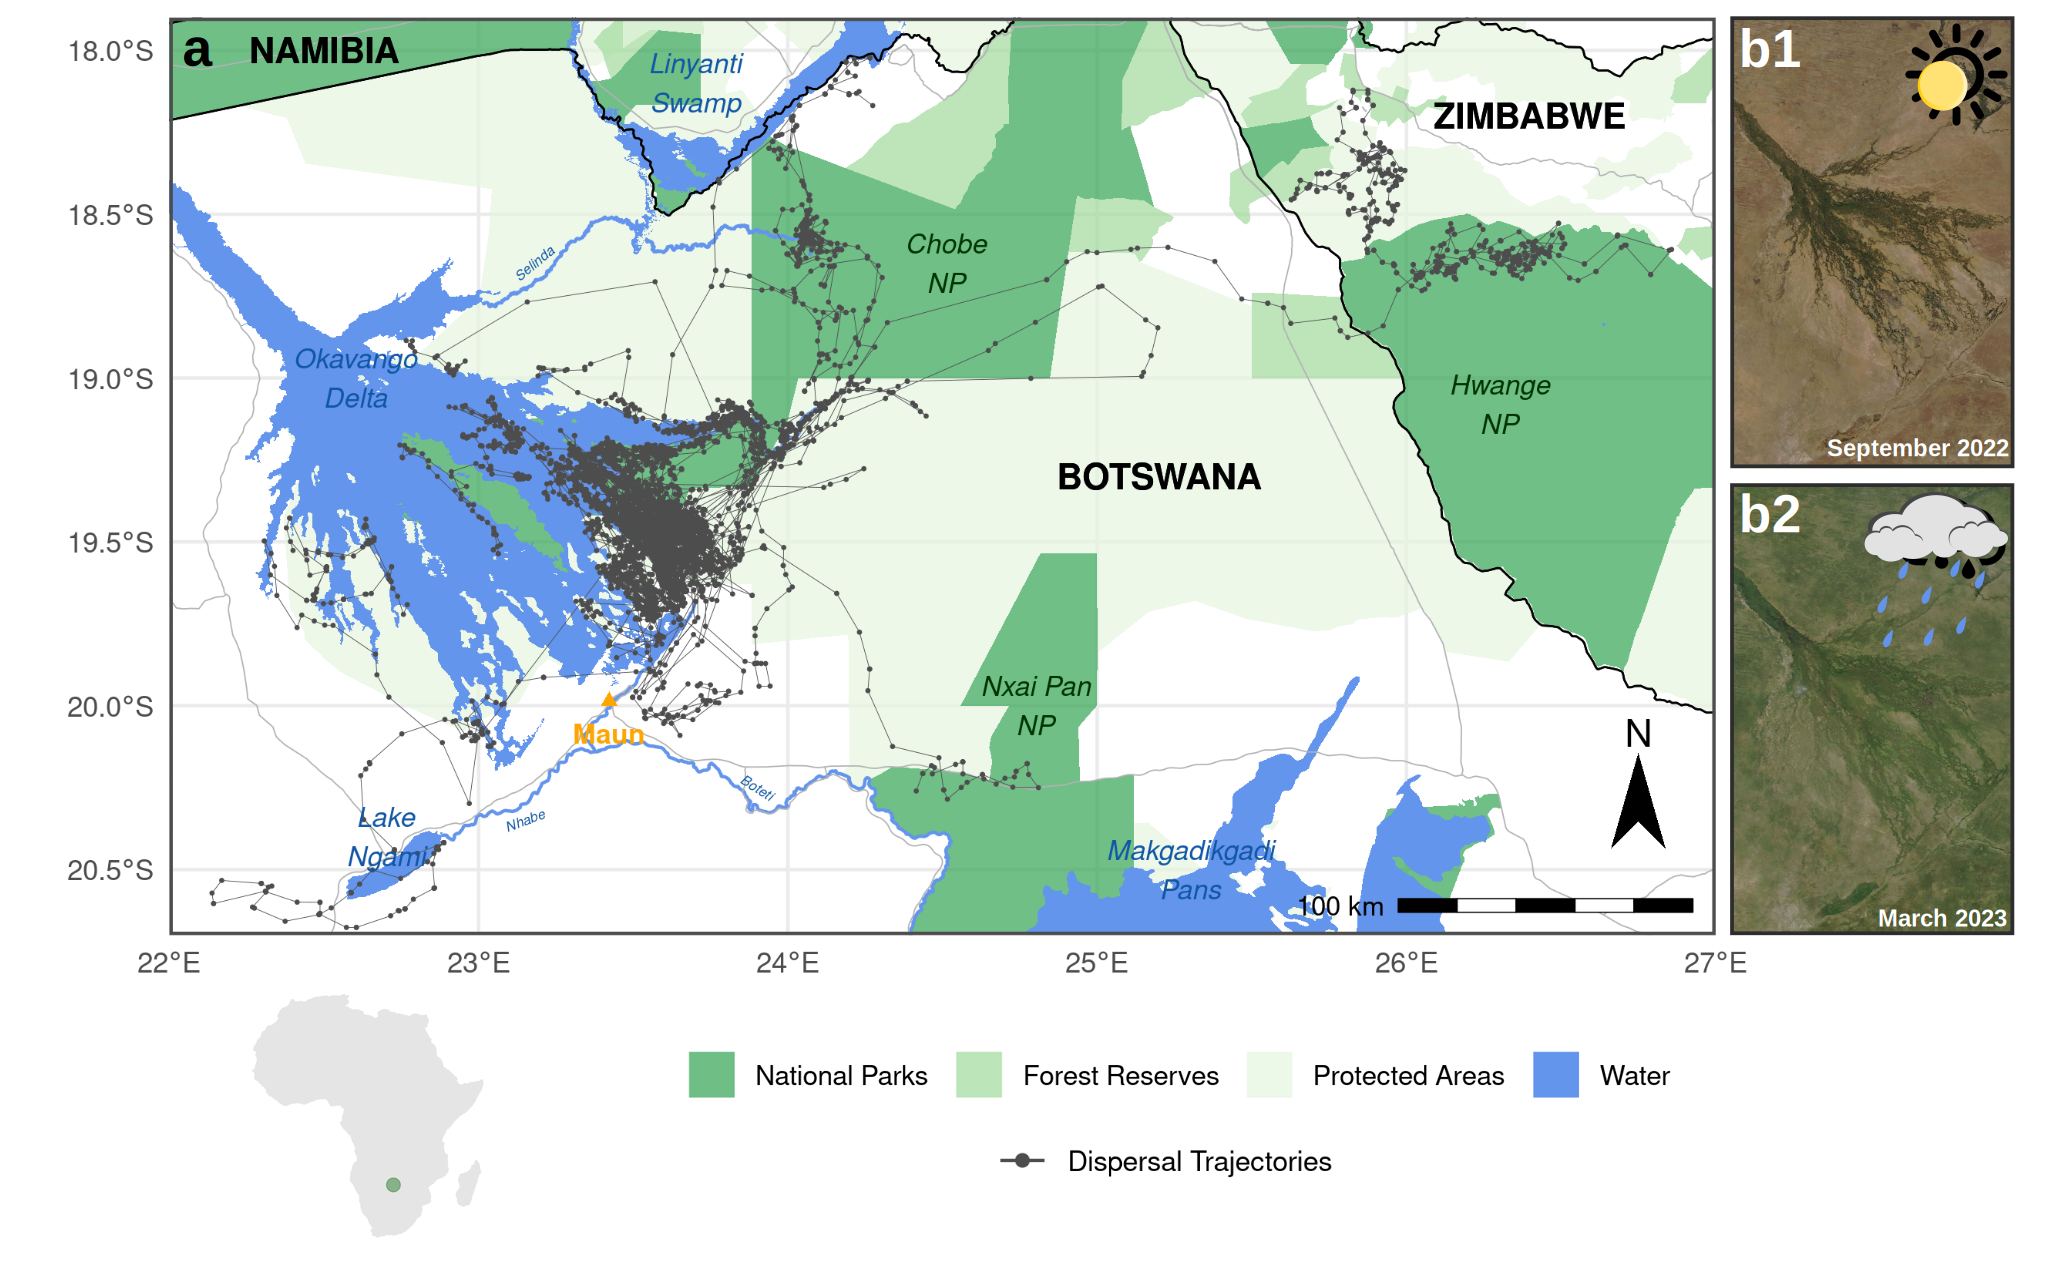
\includegraphics[width = \textwidth]{Figures/StudyArea.png} \caption{(a) Study
  area from which data on dispersing AWDs were collected. Dispersal trajectories
  are plotted in dark gray. The study area encompassed parts of the Okavango
  Delta in northern Botswana, a highly dynamic, flood-pulse-driven ecosystem.
  The entire study area undergoes substantial seasonal changes, as can be seen
  from two satellite images taken during peak dry season (b1) and peak rainy
  season (b2). Notably, the flood of the Okavango Delta reaches its maximum
  extent during peak dry season (August - September).}
  \label{StudyArea}
 \end{center}
\end{figure}

\subsection{GPS Data}

Between the years \inputy{GeneralMetrics/GPSFromYear} and
\inputy{GeneralMetrics/GPSToYear}, we collected GPS data of
\inputy{GeneralMetrics/CollarsTotal} dispersing AWD coalitions
(\inputy{GeneralMetrics/CollarsFemales} female coalitions,
\inputy{GeneralMetrics/CollarsMales} male coalitions) from a free-ranging
population in northern Botswana. Details on the GPS collar fitting procedure and
how we distinguished between dispersal and resident movements can be found in
\citet{Cozzi.2020} and \citet{Hofmann.2021}. During dispersal, GPS satellite
collars recorded a GPS location every four hours and regularly transmitted the
data to a base-station via Irridium satellite. In total, we successfully
collected \inputy{GeneralMetrics/FixesTotal} locations during dispersal, with an
average of \inputy{GeneralMetrics/FixesMeanSD} locations per coalition.
Occasionally, the acquisition of a GPS location failed (success rate =
\inputy{GeneralMetrics/AcquisitionRate}\%), resulting in slight deviations from
the aspired four-hourly interval.

\subsection{Covariates}

We represented the physical landscape through which dispersers could move by a
suite of spatial layers that we believed would influence wild dog movements
during dispersal. The layers can be broadly categorized into descriptors of (1)
landscape characteristics, (2) climatic conditions, and (3) anthropogenic
factors (\Cref{Covariates}). Besides these spatial layers, we also prepared a
series of (4) nocturnal statistics (\Cref{Covariates}). To appropriately render
seasonality in each of the spatial covariates (1-3), we downloaded spatial data
at the highest spatial and temporal resolution available. Specifically, we
attempted to represented covariates by a series of raster layers that spanned
the entire range of dates for which we collected data of dispersing AWDs.
Depending on the products available, this resulted in differing spatial and
temporal resolutions (\Cref{Covariates}). To assess the importance of rendering
layers at such high temporal resolutions, we used these ``dynamic'' covariates
to compute ``static'' covariates, representing average conditions over the
entire study period. For this, we flattened each covariate-stack into a single
layer, thus removing seasonality from the spatial data entirely. The only
exception to this was the precipitation and temperature data, which instead we
flattened by hour of the day.

\begin{figure}
\begin{center}
  \includegraphics[width = \textwidth]{Figures/SeasonalCovariates.png}
  \caption{Illustration of how some of the covariates considered in this study
  vary across seasons. Data for the graphs were obtained from the (a) JAXA
  GSMaP, (b) ERA5 dataset, (c) MODIS MOD13Q1 dataset, and (d) remote sensed
  MOD43A4 satellite images. Values were extracted across the study area and
  averaged by months. Smoothing curves were fitted using GAM models with the
  \texttt{mgcv} package \citep{Wood.2011}.}
  \label{Seasonality}
\end{center}
\end{figure}

\onehalfspacing
\begin{center}
\begin{threeparttable}
  \caption{Covariates that were used in this study, including information on
  their temporal and spatial resolutions, as well as on the avenue through which
  the respective data were accessed or downloaded}
  \label{Covariates}
  
\begin{tabular}[t]{lcccc}
\toprule
Variable & \makecell[c]{Temporal\\Resolution} & \makecell[c]{Spatial\\Resolution} & Source & \makecell[c]{Download\\Method}\\
\midrule
\addlinespace[0.3em]
\multicolumn{5}{l}{(1) Landscape Characteristics}\\
\hspace{1em}Trees & 1 year & 250 m & MODIS MOD44B & \texttt{RGISTools}\\
\hspace{1em}Shrubs / grassland & 1 year & 250 m & MODIS MOD44B & \texttt{RGISTools}\\
\hspace{1em}NDVI & 16 days & 250 m & MODIS MOD13Q1 & \texttt{rgee}\\
\cellcolor[HTML]{f2f2f2}{\hspace{1em}Rivers} & \cellcolor[HTML]{f2f2f2}{static} & \cellcolor[HTML]{f2f2f2}{90 m} & \cellcolor[HTML]{f2f2f2}{MERIT Hydro} & \cellcolor[HTML]{f2f2f2}{website}\\
\cellcolor[HTML]{f2f2f2}{\hspace{1em}Permanent water} & \cellcolor[HTML]{f2f2f2}{static} & \cellcolor[HTML]{f2f2f2}{30 m} & \cellcolor[HTML]{f2f2f2}{Globeland30} & \cellcolor[HTML]{f2f2f2}{website}\\
\cellcolor[HTML]{f2f2f2}{\hspace{1em}Floodwater} & \cellcolor[HTML]{f2f2f2}{8 days} & \cellcolor[HTML]{f2f2f2}{500 m} & \cellcolor[HTML]{f2f2f2}{MOD34A4} & \cellcolor[HTML]{f2f2f2}{\texttt{floodmapr}}\\
\hspace{1em}Distance to water & 8 days & 500 m & MOD43A4 & \texttt{floodmapr}\\
\hspace{1em}Pans & 5/10 days & 10 m & Sentinel 2 & \texttt{sen2r}\\
\hspace{1em}Distance to pans & 5/10 days & 10 m & Sentinel 2 & \texttt{sen2r}\\
\addlinespace[0.3em]
\multicolumn{5}{l}{(2) Climate Descriptors}\\
\hspace{1em}Temperature & 4 hours & 10 km & ERA5 & \texttt{rgee}\\
\hspace{1em}Precipitation & 4 hours & 10 km & JAXA GSMaP & \texttt{rgee}\\
\addlinespace[0.3em]
\multicolumn{5}{l}{(3) Anthropogenic Features}\\
\cellcolor[HTML]{f2f2f2}{\hspace{1em}Human density} & \cellcolor[HTML]{f2f2f2}{static} & \cellcolor[HTML]{f2f2f2}{30 m} & \cellcolor[HTML]{f2f2f2}{Facebook} & \cellcolor[HTML]{f2f2f2}{website}\\
\cellcolor[HTML]{f2f2f2}{\hspace{1em}Agriculture} & \cellcolor[HTML]{f2f2f2}{static} & \cellcolor[HTML]{f2f2f2}{30 m} & \cellcolor[HTML]{f2f2f2}{Globeland30 / Cropland} & \cellcolor[HTML]{f2f2f2}{website}\\
\cellcolor[HTML]{f2f2f2}{\hspace{1em}Roads} & \cellcolor[HTML]{f2f2f2}{static} & \cellcolor[HTML]{f2f2f2}{vectorized} & \cellcolor[HTML]{f2f2f2}{Open Street Map} & \cellcolor[HTML]{f2f2f2}{website}\\
\addlinespace[0.3em]
\multicolumn{5}{l}{(4) Light Availability}\\
\cellcolor[HTML]{f2f2f2}{\hspace{1em}Night} & \cellcolor[HTML]{f2f2f2}{4 hours} & \cellcolor[HTML]{f2f2f2}{-} & \cellcolor[HTML]{f2f2f2}{-} & \cellcolor[HTML]{f2f2f2}{\texttt{moonlit}}\\
\cellcolor[HTML]{f2f2f2}{\hspace{1em}Moon illumination} & \cellcolor[HTML]{f2f2f2}{4 hours} & \cellcolor[HTML]{f2f2f2}{-} & \cellcolor[HTML]{f2f2f2}{-} & \cellcolor[HTML]{f2f2f2}{\texttt{moonlit}}\\
\bottomrule
\end{tabular}

  \begin{tablenotes}
    \item \textit{The spatial layers in gray were combined into a single proxy
    of human influence, as described in \citet{Hofmann.2021}.}
  \end{tablenotes}
\end{threeparttable}
\end{center}
\doublespacing

\subsubsection{Landscape Characteristics}

We used data from the MODIS Vegetation Continuous Fields dataset (MOD44B V061;
\citealp{DiMiceli.2022}) to represent vegetation across the study area. The
MOD44B dataset comprised three continuous layers, depicting the percentage cover
of woodland, shrubs/grassland, and bareland, respectively. The three layers
added up to 100\%, so we dropped bareland layer to prevent perfect
multicollinearity. The MOD44B product is updated on day 65 of each year, so we
used the \texttt{R}-package \texttt{RGISTools} \citep{Perez-Goya.2020} to
download yearly updated layers. Furthermore, we downloaded information on the
normalized vegetation difference index (NDVI) from the MODIS MOD13Q1 dataset
\citep{Didan.2015}. This product is updated every 16 days, and we accessed the
respective layers through Google Earth Engine \citep{Gorelick.2017} using the
\texttt{R}-package \texttt{rgee} \citep{Aybar.2023}. To depict large, static
water-bodies, we used the Globeland30 dataset, from which we only retained the
land-cover class water, while setting all other categories to dryland.
Similarly, we used the MERIT Hydro dataset to obtain information on permanent
rivers \citep{Yamazaki.2019}. To depict large, dynamic water-bodies,
particularly the floodwaters of the Okavango Delta, we prepared weekly updated
floodmaps using remote sensed MODIS MOD43A4 satellite images. The algorithm upon
which the identification of flooded areas is based is described in detail in
\citet{Wolski.2017} and \citet{Hofmann.2021} and implemented in the
\texttt{floodmapr} package (available on GitHub;
\url{https://github.com/DavidDHofmann/floodmapr}). We also modeled small,
ephemeral water bodies (i.e., pans) by applying a customly built random forest
classifier to Sentinel 2 satellite imagery (\citealp{EuropeanSpaceAgency.2018};
details of the classifier in Appendix S1). While Sentinel 2 satellite imagery is
updated every 5 days, cloud cover often results in incomplete images, thus
prohibiting producing ``pan-maps'' at this frequency. Instead, we opted for
monthly update composite images, thus minimizing the risk of misclassification
due to cloud cover. The procedure resulted in monthly updated pan-maps that
depicted the distribution of ephemeral waterbodies as small as a few meters
(Appendix SX).

\subsubsection{Climate Descriptors}
We used hourly updated information on above-ground temperature from the
ERA5-Land dataset \citep{Munoz-Sabater.2021} and hourly updated precipitation
estimates from the Global Satellite Mapping of Precipitation dataset
\citep{Kubota.2020}. Both datasets were accessed and downloaded through Google
Earth Engine \citep{Gorelick.2017} using the \texttt{rgee} package
\citep{Aybar.2023}. To match hourly values from the temperature and
precipitation data with the 4-hour fixes from the GPS data collection, we
computed average precipitation and temperature values across four hours.

\subsubsection{Anthropogenic Features}

We combined anthropogenic pressures arising from the presence of humans,
agriculture, and roads into a single proxy for human influence. We obtained
information on human density from Facebook's high resolution human density
dataset \citep{Tiecke.2017} which we downloaded from the humdata website
(\url{www.data.humdata.org/}). Likewise, we obtained information on the presence
of agricultural fields from the Globeland30 \citep{Chen.2015} and Cropland
\citep{Xiong.2017} datasets. We downloaded on main tar roads from OpenStreetMaps
\citep{OpenStreetMapContributors.2017}. We combined the different features into
a single layer according to the rules described in \citet{Hofmann.2021}.
Finally, we derived vector data on the distribution of national parks, wildlife
management areas and other protected areas from the Peace Parks Foundation
(\url{www.maps.ppf.org.za/}).

\subsubsection{Nocturnal Variables}

We calculated nocturnal covariates associated with each step using the
\texttt{moonlit} package \citep{Smielak.2023}. The set of covariates included a
binary variable indicating if a step fell into daytime or nighttime (sun $<$ -18
\degree below the horizon), a variable of the moon phase (fraction of the
visible moon relative to full-moon), and an estimate of moonlight illumination
(in lux).

\subsection{Step-Selection Models}

We modeled the habitat and movement preferences of dispersing individuals using
integrated step-selection functions (iSSFs, \citealp{Fortin.2005, Avgar.2016}),
following the procedure described in \citet{Muff.2020}. For this, we first
identified bursts of subsequent GPS locations where the duration between two
recordings did not exceed 4 hours (\(\pm\) 15 minutes). Within each burst, we
converted locations into steps, where a step represented the straight line
between two consecutive locations \citep{Turchin.1998}. For each step, we
computed the associated step-length (sl, in kilometers) and turning-angle (ta,
in radians) relative to the preceding step. Due to the 4-hour regularization,
some individuals dropped from the final dataset, leaving data of
\inputy{GeneralMetrics/SSFTotal} dispersing coalitions
(\inputy{GeneralMetrics/SSFFemales} female coalitions,
\inputy{GeneralMetrics/SSFMales} male coalitions) to work with. The final
dataset comprised \inputy{GeneralMetrics/StepsTotal} steps
(\inputy{GeneralMetrics/StepsMeanSD} per coalition), which we further
categorized into wet and dry season. This resulted in
\inputy{GeneralMetrics/NumberStepsDry} steps
(\inputy{GeneralMetrics/PercentageStepsDry}\%) during the dry season and
\inputy{GeneralMetrics/NumberStepsWet} steps
(\inputy{GeneralMetrics/PercentageStepsWet}\%) during the wet season.

We paired each \textit{observed} step with a set of 100 \textit{random} steps,
generated by sampling turning angles from  a uniform distribution U(\(-\pi,
+\pi\)) and step lengths from a gamma distribution fitted to observed steps
(scale \(\theta\) = \inputy{GeneralMetrics/GammaScale} and shape \(k\) =
\inputy{GeneralMetrics/GammaShape}). Together, an observed step and its 100
associated random steps formed a stratum that received a unique identifier.
Along each step, we extracted covariate values from the underlying spatial
habitat layers (\Cref{Covariates}). For continuous covariates, we computed
average values along each step, for categorical covariates the percentage cover
of each category along the step. To model a decreasing marginal impact of
``distance to'' variables, we included their square-root as predictors. To
facilitate model convergence, we normalized resulting values to a range between
0 and 1. To estimate habitat and movement parameters of interest, we applied the
maximum likelihood procedure proposed by \citet{Muff.2020}, using the
\texttt{glmmTMB} package \citep{Brooks.2017}. We included a stratum-specific
intercept with a fixed and large variance ($10^6$), and used dispersing
coalition ID to model random slopes.

Talk about the model structure here...

To establish whether 100 random steps sufficed to reliably estimate parameters,
we ran a series of univariate models where we only included single covariates
and estimated model coefficients considering 1, 5, 10, 50, 75, and 100 random
steps, respectively (sensu \citealp{Fieberg.2021}). We replicated each model 100
times using randomly resampled steps and we computed the deviation of the
resulting estimate to the estimate emerging under the maximum of 100 random
steps. The results confirmed that model estimates stabilized at ca. 25 random
steps, suggesting that 100 random steps were well beyond sufficient (Figure S8).

Ultimately, we parametrized four models that differed in their degrees of
dynamism in two dimensions, as outlined in (\Cref{GraphicalAbstract}a). Models
one and two were both fit using static covariates (\Cref{GraphicalAbstract}a),
with model one being a single-season model, model two being a two-season model
(wet vs. dry). Models two and three, by contrast, were fit using dynamic
covariates, with model three being a single-season model, and model four being a
multi-season model (wet vs. dry). To fit these models, we used data of 20
individuals ($\sim$ 80\%), retaining the remaining six ($\sim$ 20\%) for
validation purposes.

% created xx candidate models that we ranked based on Akaike's Information
% Criterion (AIC, \citealp{Akaike.1974, Burnham.2002}).

\subsection{Simulation}

Using the four parameterized iSSF models we simulated utilization distributions
(UDs) for each individual in the validation dataset, either assuming a static or
a dynamic landscape (\Cref{GraphicalAbstract}). Each of the retained individuals
dispersed during a different time and from a different origin, which is why we
simulated separate utilization distributions for each individual. For the
simulation, we employed the iSSF-simulation-framework introduced by
\citet{Signer.2017} and employed in \citet{Hofmann.2023}. The procedure starts
by selecting a start-point, which in our case was set at the first location of
an individual's dispersal track. Originating from this location, we then
proposed a set of random steps by sampling turning-angles from the fitted gamma
distribution and turning-angles from a von Mises distribution. Along each of the
so created random steps, we extracted spatial covariates and computed relevant
movement metrics (sl, log(sl), and cos(ta)). We then employed the fitted
model(s) to predict the likelihood of each step for being chosen (i.e. the
redistribution kernel) and sampled one of the steps based on assigned
probabilities. We then updated the simulated individual's position and repeated
the procedure until the number of simulated steps matched that of the observed
individual. We repeated the simulation 20'000 times for each configuration. For
configurations in which the covariates were updated dynamically \textit{during}
the simulation, we generated a new set of covariate layers after every step,
thus rendering conditions as up to date as possible (\Cref{Schematic}). For all
configurations, we finally obtained utilization distributions (heatmaps) base on
simulated locations.

\begin{figure}
 \begin{center}
  \includegraphics[width = \textwidth]{Figures/Schematic} \caption{Schematic
  illustration of the dispersal simulation with dynamic covariates. As the
  simulation proceeded, we updated underlying environmental conditions
  (symbolized by the stack of layers). To update the covariate stack, we
  utilized series of seasonally updated spatial layers (each grey bars along the
  timeline indicates a new layer). Depending on the covariate, the update
  frequency ranged from a few hours to multiple months. We then proposed a set
  of random steps and applied the parametrized step-selection function to
  generate a redistribution kernel, indicating the probability of each step for
  being chosen. Based on this kernel, one location was sampled and the animal's
  position updated. This procedure was repeated until the number of simulated
  steps matched the number of steps from the observed individuals.}
  \label{Schematic}
 \end{center}
\end{figure}

\subsection{Validation}

To assess the predictive efficacy of each configuration, we employed
the validation dataset and ran a step-selection function, establishing whether
individuals contained within this dataset systematically favored areas of high
predicted utilization. Specifically, we overlaid each of the simulated
utilization distributions with the true, observed dispersal tracks and computed
the average utilization value along each observed and random steps and used a
conditional logistic regression to estimate the selection coefficient
$\beta_{UD}$. Our rationale was that this value should be higher, the better a
model predicted the true dispersal movements.

\section{Results}

\begin{figure}
 \begin{center}
  \includegraphics[width = \textwidth]{Figures/MovementModel.png}
  \caption{This is a caption}
  \label{Movement Model}
 \end{center}
\end{figure}

\inputy{Figures/MovementModel.tex}

\section{Discussion}
Dynamic connectivity increases our understanding of temporal changes in
connectivity \citep{Martensen.2017}.

\citet{Martensen.2017} showed that dynamic connectivity was higher than static
connectivity because of stepping stones that emerged and disappeared again.

\citet{Osipova.2019} in contrast find that connectivity is both over and
underestimated, depending on the season.

\citet{Benz.2016} showed that habitat selection of moose changes depending on the
season and used a combination of RSFs and SSFs to study habitat selection across
seasons.

Badly designed corridors can result in population sinks and wasted financial
resources \citep{Simberloff.1992}.

Could talk a bit about the following papers: \citep{Chetkiewicz.2009, Benz.2016,
Mui.2017, Osipova.2019, Kaszta.2021}

\section{Authors' Contributions}
D.D.H. and G.C. conceived the study and designed methodology; D.D.H., G.C.,
D.M.B, and J.W.M. collected the data; D.D.H. analysed the data; G.C. assisted
with modeling; D.D.H. and G.C. wrote the first draft of the manuscript and all
authors contributed to the drafts at several stages and gave final approval for
publication.

\section{Data Availability}
Something

\section{Acknowledgements}
Something

\newpage
\begingroup
\singlespacing
\ifthenelse{\boolean{usebiblatex}}{
  \begin{refcontext}[sorting=nyt]
  \printbibliography
  \end{refcontext}
}{
  \bibliography{LiteratureBibtex}
}
\endgroup
\end{document}
